%
% Niniejszy plik stanowi przyk³ad formatowania pracy magisterskiej na
% Wydziale MIM UW.  Szkielet u¿ytych poleceñ mo¿na wykorzystywaæ do
% woli, np. formatujac wlasna prace.
%
% Zawartosc merytoryczna stanowi oryginalnosiagniecie
% naukowosciowe Marcina Wolinskiego.  Wszelkie prawa zastrze¿one.
%
% Copyright (c) 2001 by Marcin Woliñski <M.Wolinski@gust.org.pl>
% Poprawki spowodowane zmianami przepisów - Marcin Szczuka, 1.10.2004
% Poprawki spowodowane zmianami przepisow i ujednolicenie
% - Seweryn Kar³owicz, 05.05.2006

\documentclass[licencjacka]{pracamgr}

\usepackage{polski}

\usepackage[utf8]{inputenc}

\usepackage{pdfpages}

\usepackage{gensymb}

\usepackage{url}

% Dane licencjanta:

\author	{Imię Nazwisko}

\nralbumu{666999}

\title{Implementacja taktycznej gry fabularnej czasu rzeczywistego}

\tytulang{An implementation of a real-time strategy role-playing game}

\kierunek{Informatyka}

\opiekun{mgra Radosława Bartosiaka\\
  Instytut Informatyki\\
  }

% miesiąc i rok:
\date{Maj 2015}

\dziedzina{11.3 Informatyka}

%Klasyfikacja tematyczna wedlug ACM (informatyka)
\klasyfikacja{D. Software}

\keywords{gra, gra komputerowa, qt, sfml, box2d, taktyczna gra fabularna}

% Tu jest dobre miejsce na Twoje własne makra i środowiska:
% \newtheorem{defi}{Definicja}[section]

% koniec definicji

\begin{document}
\maketitle

%tu idzie streszczenie na strone poczatkowa
\begin{abstract}
  Niniejsza praca opisuje taktyczną grę fabularną stworzoną
  w~ramach przedmiotu Zespołowy Projekt Programistyczny.
  W~szczególności opisane zostało projektowanie silnika,
  mechaniki oraz~interfejsu gry. Praca zawiera również
  opis osiagniętego rezultatu wraz z~wynikiem przeprowadzonych testów.
\end{abstract}

\tableofcontents
%\listoffigures
%\listoftables

\chapter*{Wprowadzenie}
\addcontentsline{toc}{chapter}{Wprowadzenie}
Cyfrowa rewolucja, dziejąca się od kilkudziesięciu lat, zmieniła niemal każdy aspekt życia współczesnego człowieka.
Interesującym jest fakt, iż tak potężny i przełomowy wynalazek jakim jest komputer, do domów wielu zjadaczy chleba
zawitał po raz pierwszy jako zabawka, urządzenie mające zapewniać prostą rozrywkę. Współczenie, przemysł
gier komputerowych, którego wartość szacuje się na ok. 100 miliardów dolarów, wciąż zyskuje na popularności.
Pomimo setek tysięcy wyprodukowanych gier, zaangażowania wielkich koncernów, wciąż istnieje na rynku zapotrzebowanie
na nowe, oryginalne produkcje, które dostarczą graczowi niezapomnianych przeżyć i przykują go do komputera na długie godziny.

Z punktu widzenia twórcy, gry komputerowe stanowią jednak niezwykle trudne wyzwanie. Po pierwsze, należy stawić czoła
nieprzeciętnym problemom technicznym, wymagającym wszechstronnej wiedzy informatycznej, pozwalającej do maksimum wykorzystać
dostępne medium. Po drugie, gry wymagają szerokiej wiedzy z przeróżnych dziedzin, związanych z
grafiką, dźwiękiem, tworzeniem fabuły. W końcu, należy te wszystkie składniki połączyć, mając przed sobą ostateczny cel: dostarczenie
graczowi wysokiej jakości rozrywki. Skomplikowanie i trudność w sprecyzowaniu tego celu powodują, że proces tworzenia gier
znacząco różni się od produkcji innego rodzaju oprogramowania. Dopiero harmonijne zgranie wszystkich składników, podporządkowanie
ich spójnej wizji, ma szansę wywołać u gracza niezapomnianie przeżycia i zapewnić twórcy pełną satysfakcję z wykonanej pracy.

Poniższy tekst opisuje zrealizowany przez nas projekt silnika gry komputerowej, wraz~z~przykładową implementacją gry. W kolejnych
rozdziałach prezentujemy główne ograniczenia projektowe, opis założonego produktu końcowego,
techniczne aspekty realizacji projektu, uzyskane rezultaty i wnioski z naszej rocznej pracy.


\chapter{Słownik}
  \paragraph{Decale} efekty wizualne (np. ślad po strzale, ślad krwi) rysowane na powierzchni oteksturowanego już obiektu.
  Wykorzystywane w grach, aby dodać np. dziurę po strzale, ślad krwi, symbol, dodatkowy element wizualny itp.

  \paragraph{Fog of War (,,mgła wojny'', FOW)} zaciemniony, a tym samym niewidoczny dla gracza obszar na mapie gry. Wyróżniamy:
  \begin{itemize}
   \item pierwszy stopień - obszar zupełnie niewidoczny (na czarno),
   \item drugi stopień - obszar częściowo przesłonięty, na którym widać mapę i statyczne obiekty, ale
      nie widać jednostek
  \end{itemize}

  \paragraph{Tile} ,,kafelek'', logiczny atomowy element budujący podłoże mapy, będący kwadratem o boku ustalonego rozmiaru. Całą
  mapę da się zawsze podzielić na tile danego rozmiaru - wtedy wszystkie tile podziału są takich samych rozmiarów oraz
  cała mapa jest podzielona.

  \paragraph{Playtesty} proces tworzenia gry, podczas którego twórcy testują grę w poszukiwaniu błędów,
  wad projektowych mechaniki lub interfejsu zanim gra trafi na rynek.
  \paragraph{Content gry} ogólne określenie na wszelkie elementy gry, niebędące częścią programu. Zwykle do contentu zalicza się
  dźwięk, grafikę, wyświetlane teksty, parametryzację gry.
  \paragraph{Silnik gry} system informatyczny udostępniający gotowe funkcjonalności, potrzebne do implementacji gry komputerowej.

\chapter{Projekt}

  \section{Opis projektu}
% Tutaj o tym, że to na ZPP i dla ProGier
  Zgodnie z zamówieniem klienta, realizowany projekt miał polegać na stworzeniu gry komputerowej
  średnich rozmiarów. Ze względu na skład zespołu, złożonego wyłącznie z programistów, skupiliśmy się
  na dostarczeniu rozbudowanego, w pełni funkcjonalnego silnika gry.
  Docelowa aplikacja miała być grywalnym produktem, prezentującym możliwości zaimplementowanego silnika,
  bez contentu i grafiki na poziomie konkurencyjnych, komercyjnych gier. Dodatkowym wymogiem było zrealizowanie
  projektu, w sposób umożliwiający dystrybucję na wielu systemach operacyjnych (Windows, Linux). Aby uniknąć
  tworzenia wielkiej gry bez możliwości ukończenia jej w realistycznym czasie, silnik miał być łatwo skalowalny
  i pozwolić na realizację zarówno małych jak i całkiem dużych gier.

  \section{Założenia projektowe}
  W pierwszej fazie projektu wybrana została ogólna koncepcja gry, z której wynikają dalsze postanowienia dotyczące
  tworzonego silnika. Zdecydowaliśmy się na realizację gry taktycznej, czasu rzeczywistego. Rola gracza ma polegać
  na sterowaniu niewielką grupą unikalnych postaci i realizowaniu kolejnych misji. Postęp gry jest wynikiem kończenia
  kolejnych, powiązanych ze sobą poziomów. Każdy z nich może wprowadzać pewne wątki fabularne. Poza głównymi zadaniami,
  decydującymi o zakończeniu misji sukcesem, gracz może realizować także zadania poboczne, nie mające wpływu na
  postęp fabularny gry. Główną trudnością ma być utrzymanie postaci przy życiu, podczas ataków wrogich jednostek.
  Mechanika systemu powinna skłaniać gracza do przemyślanych, taktycznych działań, bez testowania jego zdolności
  szybkiego klikania. Równocześnie staramy się uniknąć zbyt pasywnej postawy użytkownika.

  \section{Grupa docelowa}
  Aby uzyskać jak najwięcej informacji zwrotnych na temat naszego systemu, postanowiliśmy skierować nasz system do
  graczy komputerowych zainteresowanych grami taktycznymi, wymagającymi myślenia. Głównym źródłem satysfakcji
  odbiorcy ma być ciekawa mechanika i rozwiązywanie problemów strategicznych. Wyzwania gry powinny być realizowane przez
  odpowiednią konstrukcję poszczególnych poziomów i konieczność dostosowywania się do zmiennej sytuacji na planszy.

  \section{Osadzenie rozgrywki}
  Gra osadzona jest w niedalekiej przyszłości, około roku 2050, w świecie lekko fantastycznym, wzorowanym na
  rzeczywistym. W wyniku silnych ruchów tektonicznych na terenie Australii, ujawniony zostaje rodzaj tunelu
  prowadzącego w głąb Ziemi. Organizacje międzynarodowe decydują się wysłać ekspedycję, która zbada to niezwykłe
  zjawisko. Pierwsza ekspedycja odkrywa gigantyczne kompleksy jaskiń, które wyglądają na stworzone przez człowieka.
  Po dalszych badaniach odkrywają, że głębsze jaskinie są zamieszkane przez rasę nieznaną ludzkości. Niedługo
  po tym odkryciu, kontakt z pierwszą ekspedycją urywa się. Pod wpływem tych niecodziennych zdarzeń, najróżniejsze
  instytucje decydują się na podjęcie badań na własną rękę. Jak się okazuje, podobne tunele istnieją na całym świecie,
  ukryte w najdziwniejszych miejscach. Dopiero ostatni skok technologiczny pozwolił na ich wykrycie. Wysłana zostaje
  druga oficjalna ekspedycja, której przewodził będzie gracz. Po osiągnięciu pewnej głębokości, zaczynają pojawiać się
  problemy z łącznością. Kontakt z powierzchnią jest rzadki i zakłócony. Po dotarciu do pierwszych, pustych już zabudowań
  dziwnej cywilizacji, ekspedycja dzieli się na dwie części, bazę badawczą, która pozostaje na miejscu i ma umożliwić
  pracę drugiej części, która zapuszcza się głębiej. Dość szybko druga część zostaje zaatakowana przez nieznane stwory,
  które mordują większość członków ekspedycji i odcinają możliwość powrotu. Gracz wciela się w dowódcę odciętego
  oddziału, który musi poradzić sobie z trudną sytuacją i odkryć, co stało się z pierwszą wyprawą i kim są nieznane
  stwory. Członkowie wyprawy szybko zauważają, że nie są jedynymi, którzy postanowili zbadać podziemne miasta.

  \section{Mechanika}
    \subsection{Rola gracza}
    Gracz steruje jednym oddziałem poruszającym się po zabudowanych, wielkich kompleksach jaskiń. Powoli przenosząc
    swój obóz i zabezpieczając się przed atakami, oddział musi poruszać się do przodu, aby realizować kolejne, stawiane
    sobie zadania. Gracz może kazać każdemu z członków ekspedycji przemieszczać się po planszy, przejmować budynki lub
    tworzyć prowizoryczne konstrukcje obronne. Oprócz tego, zarządza ich ekwipunkiem i wydaje rozkazy dotyczące reagowania
    na zagrożenie. Ze względu na braki żywności i rosnące zagrożenie, gracz musi wykonywać misje szybko, starając się
    nie stracić taktycznej przewagi nad otaczającymi go wrogimi jednostkami.

    \subsection{Elementy gry}
    \paragraph{Plansza}
      Każdy level jest rozgrywany na osobnej planszy, przedstawiającej jakiś fragment podziemia, zamieszkałego przez
      obcą cywilizację. Składa się ona z grafiki tła, ścian jaskiń i umieszczonych w wolnych przestrzeniach obiektów gry.
    \paragraph{Budynki}
      Jednym z najważniejszych elementów gry są budynki. Służą one graczowi do przejmowania taktycznej przewagi na danym
      terenie, umożliwiając skuteczniejszy ostrzał okolicy i pozwalając bezpiecznie przechować swoje jednostki. Oprócz tego,
      w budynkach znajdują się różnego rodzaju przedmioty.
    \paragraph{Konstrukcje obronne}
      Konstrukcje obronne są obiektami tworzonymi i stawianymi na planszy przez postaci. Służą poprawieniu sytuacji
      taktycznej gracza na danym obszarze. Niektóre z nich, mogą wymagać do swego działania operatora – postaci która
      do nich ,,wejdzie''. Konstrukcje są budowane przez postaci z elementów znalezionych w budynkach. Konstrukcje mogą
      zostać złożone i przeniesione w nowe miejsce.
    \paragraph{Postaci}
      Postaci reprezentują pojedynczych członków ekspedycji. Mogą oni należeć do ekspedycji dowodzonej przez gracza,
      wtedy ma on nad nimi kontrolę, lub innej, dowodzonej przez AI. Każda z postaci posiada stały zestaw Umiejętności,
      wpływających na sprawność wykonywania konkretnych działań, Atrybutów, będących stałymi parametrami, niewpływającymi
      na wykonywanie czynności oraz Opis, krótko informujący gracza o osobistych cechach danej jednostki. Postać w danej
      chwili posiada także pewien Ekwipunek, Nastawienie oraz Stan. Niektóre wartości opisujące Stan są dynamicznie wyliczane,
      inne nie. Nastawienie jest parametrem ustawianym bezpośrednio przez gracza i mówi, jak dana postać reaguje na jednostki
      neutralne i wrogie. Postaci mogą chodzić po niezajętych przestrzeniach miejskich, przenosić konstrukcje obronne,
      przejmować budynki, sterować konstrukcjami obronnymi, walczyć ze sobą nawzajem i z tubylcami. W celu urozmaicenia
      gameplay'u, dążymy do możliwie dużej różnorodności w parametryzacji Umiejętności i Atrybutów postaci, tak aby każda
      z nich mogła mieć ciekawą, osobną historię fabularną i była użyteczna dla gracza w nieco inny sposób. Dzięki temu
      tworzymy wyraźne role poszczególnych postaci (medyk, inżynier, żołnierz, zwiadowca). Początkowo, każda z postaci
      ma ekwipunek, który został dla niej zdefiniowany na etapie tworzenia levelu.
    \paragraph{Tubylcy}
      Tubylcy są jednostkami podobnymi do postaci, w sensie zachowania na planszy. Wszyscy są sterowani przez proste AI.
      Posiadają tylko jeden rodzaj nastawienia, agresywny. Poruszają się w sposób mniej więcej losowy po całej planszy,
      atakując wszelkie spotkane postaci, niezależnie od tego, do jakiej należą one ekspedycji. Początkowo,
      niektórzy tubylcy mogą znajdować się w budynkach i wyjść z nich dopiero, kiedy ktoś się zbliży. Poziomy Atrybutów,
      Umiejętności i Ekwipunek poszczególnych Tubylców są generowane pół losowo na etapie tworzenia mapy.
    \paragraph{Przeszkody stałe}
      Przeszkody stałe są niezniszczalnymi elementami mapy. Tworzone są na poziomie edytowania levelu i nie udostępniają
      graczowi żadnej możliwej interakcji. Są nieruchomymi, nieprzepuszczalnymi obiektami fizycznymi, takimi jak: pomnik,
      ściana skalna, ruiny.
    \paragraph{Obozy}
      Obóz ekspedycji jest podstawowym obiektem dla każdej wyprawy. To w nim znajdują się zapasy pożywienia, to w nim tworzy
      się konstrukcje obronne i do niego trafiają wszystkie znalezione w budynkach przedmioty. Interakcja postaci z obozem
      możliwa jest tylko, gdy znajduje się ona odpowiednio blisko. Jest ona wtedy automatycznie leczona i regeneruje się
      jej zdrowie psychiczne. Obozy, tak jak konstrukcje obronne, mogą być składane i przenoszone w inne miejsce. W tym czasie,
      niemożliwe jest korzystanie z ich zawartości. Zniszczenie obozu automatycznie powoduje spadek ilości pożywienia danej
      ekspedycji do 0, co kończy się śmiercią głodową wszystkich postaci, o ile nie zdążą one wykonać swojej misji.
    \paragraph{Przedmioty}
      Przedmioty w grze mogą znajdować się w jednym z 3 miejsc: w budynku (przed znalezieniem), w ekwipunku bazy lub w
      ekwipunku konkretnej postaci. Dzielimy je na 3 główne kategorie: przedmioty użytkowe, elementy do tworzenia konstrukcji
      obronnych, złożone konstrukcje.

    \subsection{Główne mechanizmy gry}
    \paragraph{Poruszanie się}
      Jedynymi mobilnymi elementami na planszy są jednostki: postaci gracza i tubylcy. Zdecydowaliśmy sie na automatyczne
      przemieszczanie się do określonego punktu docelowego. Jednostka chcąca wykonać jakąś akcję, automatycznie znajduje
      ścieżkę, którą musi iść, aby móc ją zrealizować. W ten sposób gracz może skupić się wydawaniu poleceń, które faktycznie mają
      znaczenie taktyczne, zamiast kontrolować każdy krok swoich postaci. Wyliczone ścieżki omijają wszelkie statyczne obiekty, jednak
      nie biorą pod uwagę innych jednostek. Zdecydowaliśmy, że wystarczającym rozwiązaniem będzie ,,przepychanie się'' jednostek między sobą,
      co w łatwy sposób zapewnia silnik fizyczny.
    \paragraph{Walka}
      Mechanika walki zaimplementowana w silniku jest dość skomplikowana. Kiedy jednostka decyduje się zaatakować inny obiekt,
      sprawdzane są parametry broni i jej gotowość do strzału. Broń może nie być gotowa jeśli dopiero co oddano z niej strzał lub gdy
      jest w trakcie przeładowywania. Następnie, na podstawie parametrów broni i umiejętności postaci wyliczany jest tor lotu pocisku.
      Jeśli trafiona miałaby być zaprzyjaźniona jednostka, to strzał jest anulowany. W przeciwnym przypadku, trafionemu obiektowi zadawane są
      obrażenia. Mogą być one znacząco zmodyfikowane przez jego parametry i wyposażenie. Dodatkowym bonusem zarówno do obrony jak i zdolności
      ataku jednostki jest przebywanie w budynku. Jeśli trafiony jest budynek, w którym znajduje się wiele jednostek, losowane jest, która
      zostanie trafiona.
    \paragraph{Nastawienie}
      Aby uniknąć konieczności ciągłego monitorowania wszystkich jednostek i ręcznego wydawania poleceń ataku, jednostki posiadają pewien
      stopień samodzielności zachowania. To, co jednostka może sama zrobić, jest określane przez jej nastawienie. Może być ono agresywne
      (atakuj wszystkie wrogie jednostki w zasięgu wzroku, w razie potrzeby ścigaj) lub defensywne (atakuj tylko gdy wróg podejdzie na
      odległość pewnego strzału, nie ścigaj). Zachowanie defensywne gdy jednostka znajduje się w budynku oznacza zupełną rezygnację z
      możliwości atakowania na rzecz lepszej ochrony. Jest to nastawienie które ma pomóc chronić słabe, mało bojowe jednostki, takie jak lekarz.
    \paragraph{Leczenie}
      Niektóre jednostki mogą posiadać w swoim ekwipunku różnego rodzaju przybory, służące do leczenia zaprzyjaźnionych postaci.
      Przedmioty te nie zużywają się, pozwalają na regenerowanie zdrowia w tempie zależnym od jakości przedmiotu i zdolności jednostki leczącej.
      Oprócz tego, jednostki znajdujące się blisko bazy są powoli leczone automatycznie, bez konieczności udziału lekarza.
    \paragraph{Konstrukcje obronne}
      Każda postać może przenosić różnego rodzaju konstrukcje obronne w zestawie ,,zrób to sam''. Są to różnego rodzaju barykady, bunkry, wieżyczki
      strzelnicze itp. Gracz może rozkazać jednostce postawić taką konstrukcję w wyznaczonym miejscu, co zajmuje pewien czas.
      Konstrukcje obronne mają za zadanie poprawić sytuację strategiczną gracza, gdy potrzebuje on schronić się przed wrogimi jednostkami lub
      skierować je w konkretne miejsce. Niektóre konstrukcje obronne mogą zostać złożone gdy nie są już potrzebne i przeniesione w inne miejsce.
    \paragraph{Psychoza}
      Aby zapobiec strategiom grania polegającym na ,,przebiegnięciu'' gracza przez planszę, dodaliśmy mechanizm psychozy. Postaci
      powoli tracą zdrowie psychiczne gdy znajdują się przez dłuższy czas poza bazą. Gdy spadnie ono do zera, postać wariuje i
      zaczyna się zachowywać tak jak wróg, atakując własnych sprzymierzeńców. Rozwiązaniem tego problemu jest wracanie do bazy oraz jej przenoszenie.
      Każda postać może złożyć bazę wyprawy i przewieźć ją w nowe miejsce. Sprawia to, że cała ekspedycja gracza musi w równym tempie posuwać się
      do przodu, dbając o zabezpiecznie swojej aktualnej pozycji.
    \paragraph{Głód}
      Chcąc uniknąć zbyt ostrożnego i powolnego zachowania gracza, wprowadziliśmy zjawisko głodu. Na każdej planszy, ekspedycja ma do dyspozycji pewną
      bazową ilość pożywienia. Każda postać co jakiś czas konsumuje pewną jego część. Gdy jedzenia zabraknie, jednostki dość szybko
      umierają z głodu. Mechanizm ten ma kilka ważnych konsekwencji: czasem może nie opłacać się przyjmować nowo spotkanych jednostek do ekspedycji
      (jeśli jedzą bardzo dużo), gracz musi dążyć do szybkiego wykonania zadania, czasem może opłacać się odwiedzanie jak największej liczby budynków
      tubylców, bo można w nich znaleźć dodatkowe jedzenie.
    \paragraph{Zadania}
      Na każdej planszy gracz ma do wykonania zadanie główne, które decyduje o wygraniu lub przegraniu poziomu. Oprócz niego,
      występują zadania poboczne, które mogą graczowi pomóc w zrealizowaniu zadania głównego. Każde zadanie ma pewne warunki
      rozpoczęcia, zakończenia sukcesem i zakończenia porażką. Te warunki mogą dotyczyć ilości jedzenia ekspedycji, wykonania innych zadań,
      liczby zabitych wrogów, znalezienia jakiegoś przedmiotu, zobaczenia jakiegoś obiektu, dołączenia konkretnej jednostki do ekspedycji,
      czy też wejścia do określonego budynku. O postępach w realizacji poszczególnych zadań gracz jest informowane przez specjalny system notyfikacji
      i wpisów do dziennika wyprawy.



  \section{Interfejs}
    Interfejs użytkownika naszej gry składa się z trzech głównych elementów: menu głównego, ekranu gry oraz okien wewnątrz gry.

    \subsection{Menu główne}
      Menu główne jest pierwszym miejscem do jakiego trafia użytkownik po uruchomieniu programu. Z tego miejsca może dokonać ogólnych wyborów m.in. czy
      rozpocząć nową rozgrywkę lub czy wczytać poprzednią. Menu główne jest również osiągalne podczas gry, kiedy możliwe jest także zapisanie aktualnego stanu gry.

    \subsection{Okno gry}
      Podczas gry użytkownik ma przed sobą planszę z obiektami gry, którymi zarządza przy użyciu myszki, a przy brzegach ekranu znajdują się panele,
      dzięki którym gracz wydaje część poleceń oraz poznaje stan gry. Głównym zadaniem planszy jest śledzenie stanu gry oraz zaznaczanie i wydawanie poleceń
      własnym jednostkom. Jednostki mogą być zaznaczane zarówno przez klikanie i przeciąganie myszką na mapie jak i przez użycie skrótów klawiszowych.
      Poszczególne jednostki mogą zostać wybrane dzięki klawiszom funkcyjnym (F1 - F12), a klawiszom numerycznym można przyporządkować całe grupy jednostek.
      Polecenia wydawane jednostkom dzielą się na dwie grupy:
      \begin{description}
       \item[Polecenia podstawowe] tj. atak, ruch, wejście/wyjście z lokacji
       \item[Polecenia specjalne] tj. leczenie sojusznika, postawienie/złożenie fortyfikacji lub obozu
      \end{description}
      Dokładne polecenie jakie zostanie wydane jednostkom zależy od tego, kogo gracz wcześniej zaznaczył, gdzie kliknął oraz której grupy poleceń użył.

      Poniżej zostały opisane panele, które znajdują się w oknie gry.

      \subsubsection{Panel jednostek}
      Zawiera informacje o obecnym stanie jednostek, pozwala przełączać się pomiędzy nimi oraz otwierać okno szczegółowych informacji o jednostce
      (więcej o oknie poniżej). Okna pojawiające się podczas gry nie przesłaniają nigdy tego panelu, co pozwala na kontekstową zmianę jednostek
      w zakresie danego okna (np. zamiana postaci przy oglądaniu szczegółów o jednostkach). Jest położony na górze ekranu.

      \subsubsection{Panel frakcji}
      Wyświetla podstawowe informacje o frakcji gracza i umożliwia otwieranie okien dziennika, obozu oraz wyjście do menu głównego.
      Znajduje się w prawym dolnym rogu ekranu.
      \subsubsection{Panel zachowania}
      Pozwala na zmianę zachowania obecnie zaznaczonych jednostek. Przylega do panelu frakcji.
      \subsubsection{Panel powiadomień}
      Miejsce na ekranie, gdzie pojawiają się powiadomienia o wszystkich istotnych dla użytkownika wydarzeniach gry. Jest położony w lewym górnym rogu.

    \subsection{Okna wewnątrz gry}
      \subsubsection{Okno jednostki}
      Zawiera szczegółowe informacje o wybranej jednostce gracza. Pozwala poznać jej wyposażenie, historię oraz szczegółowe statystyki i atrybuty.
      \subsubsection{Okno obozu}
      Pozwala na obejrzenie ekwipunku obozu oraz umożliwia kostruowanie nowych przedmiotów z posiadanych części.
      \subsubsection{Okno dziennika}
      Dziennik zawiera wpisy o wszystkich istotnych wydarzeniach zachodzących podczas gry. Służy do wygodnego przeglądania długich wpisów jak na przykład
      opisów aktualnych zadań.
      \subsubsection{Okno wymiany z obozem}
      Jest to specjalne okno, pojawiające się wtedy, gdy jednostka gracza odwiedzi własny obóz. Pozwala tej jednostce na wymianie własnego ekwipunku z bazą.
      Wymiana odbywa się metodą \emph{przeciągnij i upuść}.


  \section{Grafika}
    \subsection{Perspektywa}
    Świat rysowany w grze przedstawiony jest w uproszczonym wariancie perspektywy izometrycznej, często spotykanym w
    wielu produkcjach z gatunku RPG. Gdyby spojrzeć na mapę gry idealnie z góry, to aby uzyskać naszą perspektywę należy
    ją obrócić względem środka o $45\degree$, a następnie pochylić w dół o $30\degree$.

    \begin{figure}[htbp]
      \centering
      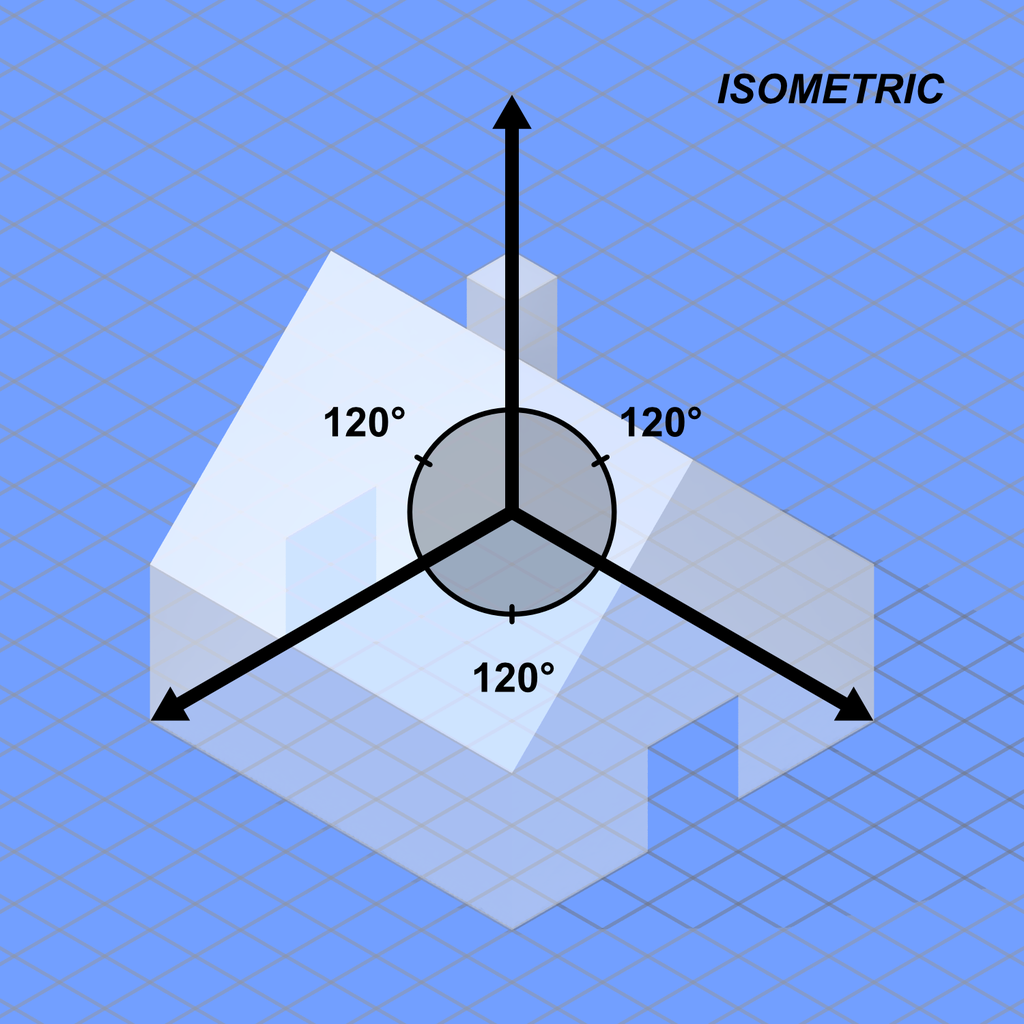
\includegraphics[scale=0.25]{izo.png}
      \caption[BLAH]{Perspektywa izometryczna\protect\footnotemark}
    \end{figure}

    \footnotetext{Grafika na licencji CC-BY-SA wykonana przez \emph{SharkD}
	  \url{http://en.wikipedia.org/wiki/File:Graphical_projection_comparison.png#/media/File:Blue_house_isometric_projection.png}}

    Przedstawienie świata w ten sposób daje wrażenie trzech wymiarów, mimo w pełni dwuwymiarowego rysowania. Tekstury
    postaci, budynków, elementów mapy i samego podłoża muszą być przygotowane w przyjętej perspektywie, ale na poziomie
    zawartości kończy się większość komplikacji. Jedną z konsekwencji przyjętego rzutu jest konieczność tłumaczenia
    współrzędnych między ekranowymi i logicznymi. Zajmuje się tym klasa Viewport z modułu UserInterface. Więcej
    informacji na ten temat znajduje się w odpowiednim rozdziale w dalszej części pracy.

    Dla lepszego imitowania trzech wymiarów, założyliśmy że każdy obiekt w grze może być zwrócony w jednym z 8 kierunków
    (co $45\degree$). Oznacza to, że (w większości przypadków) dla każdego kierunku muszą być przygotowane osobne
    grafiki.

    \subsection{Fog of War}
    Naturalną konsekwencją przyjętej perspektywy była decyzja o wprowadzeniu Fog of War. Jako że kładliśmy nacisk na
    taktyczny aspekt gry, podjęliśmy decyzję o wykorzystaniu dwustopniowej mgły - obszary nigdy nie odkryte są
    kompletnie niewidoczne, obszary obecnie poza zasięgiem widzenia, ale kiedyś już odwiedzone, są wyszarzone i nie
    widać na nich jednostek (widać natomiast obiekty statyczne).

    \begin{figure}[htbp]
      \centering
      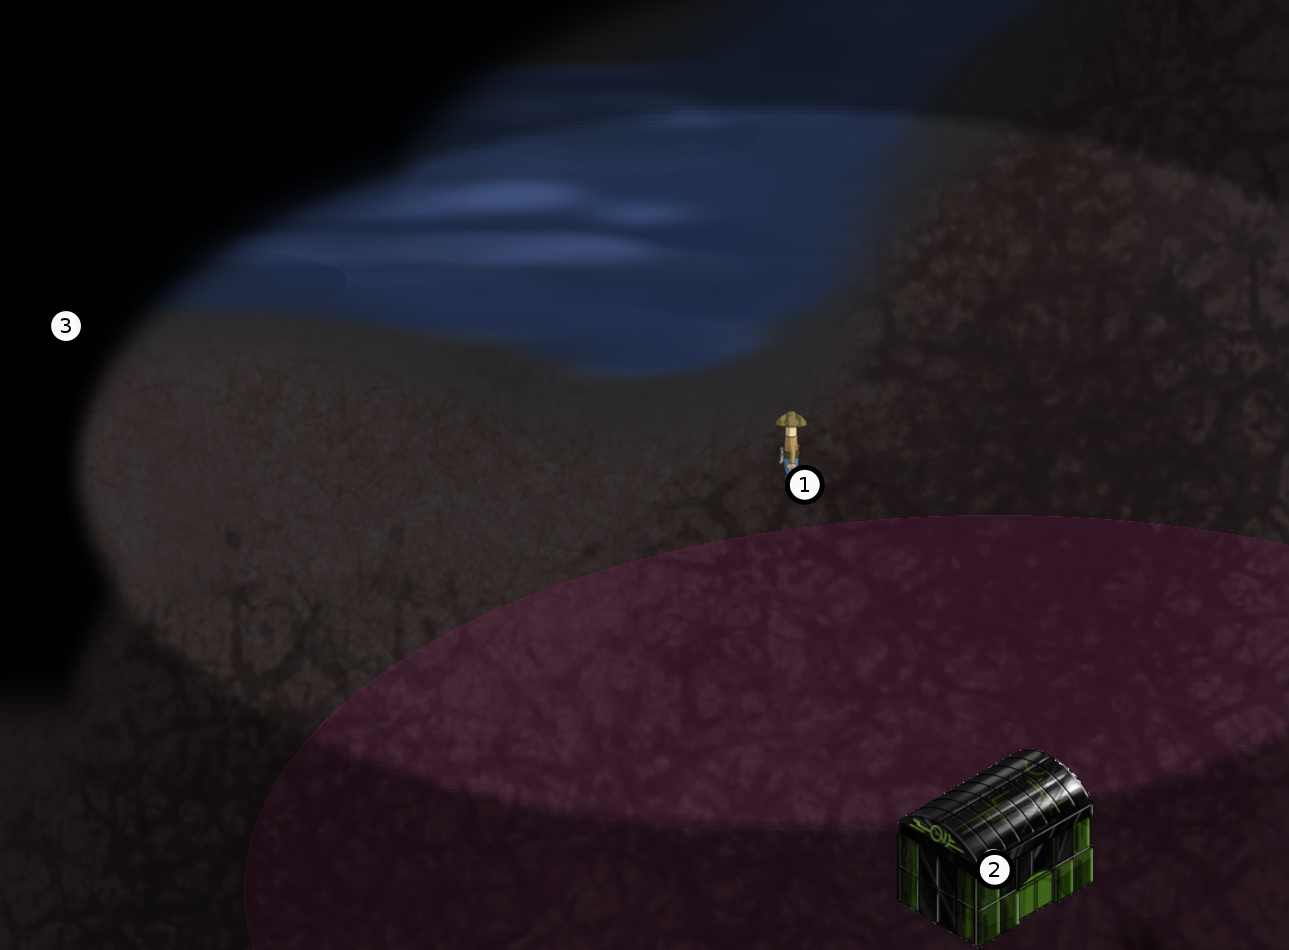
\includegraphics[scale=0.4]{fow.png}
      \caption{Fog of War w grze. 1. Jednostka, wokół której widać wszystko. 2. Baza częściowo przesłonięta przez drugi
      stopień FOW. 3. Obszar niewidoczny (pierwszy stopień).}
    \end{figure}

  \section{Analiza podobnych gier}
  Mechanika naszej gry była wymyślana od podstaw, z możliwie małą ilością zapożyczeń z innych tytułów. Możemy jednak wskazać
  kilka przykładów gier, które zawierają pewne elementy wspólne z naszym projektem.
  \subsection{Gry oparte na Commandos: Behind Enemy Lines}
    \emph{Commandos: Behind Enemy Lines} jest pierwszą grą z małego podgatunku taktycznych gier skradanych. Podobnie jak
    w naszym projekcie, gracz steruje niewielką liczbą jednostek o wyspecjalizowanych umiejętnościach i stara się wykonywać skomplikowane
    misje na planszy taktycznej, widzianej w rzucie izometrycznym. Wszystkie postaci mają indywidualną historię i są powiązane
    z fabuła gry. Inny ważnym podobieństwem jest realizacja gry w czasie rzeczywistym.

    Główna różnica polega na tym, że \emph{Commandos: Behind Enemy Lines} stawia o wiele większy nacisk na ukrywanie się postaci, unikanie walki
    i cierpliwe, długotrwałe planowanie każdego ruchu. Aby wzmocnić ten efekt, zaimplementowane zostało wykrywanie wrogich jednostek na podstawie
    słuchu, graficzne zaznaczanie pola widzenia wroga, trójkątny kształt pola widzenia, różne tempa przemieszczania się jednostek.
    My chcieliśmy uniknąć powolnej rozgrywki i zrealizować grę z większą ilością bezpośredniej, dynamicznej walki.

  \subsection{Fallout Tactics}
    Jest to kolejna gra, w której gracz steruje kilkoma, wyspecjalizowanymi jednostkami. Podobnie jak w \emph{Buried Secrets}, główny nacisk rozgrywki
    kładziony jest na strategiczną walkę i szybkie pozbywanie się wrogów. Można też wskazać podział rozgrywki na pojedyńcze zadania,
    realizowane na taktycznej mapie izometrycznej.

    Główne różnice to możliwość interakcji z innymi postaciami na ekranie (sprzedawcy), wielopoziomewe plansze, turowy tryb walki. Oprócz tego,
    w grze \emph{Fallout Tactics} gracz ma większą swobodę w wyborze postaci, którymi będzie grał i nie są one aż tak ściśle powiązane z fabułą.


\chapter{Architektura}
% tutaj dane, formaty, diagram klas, algorytmy, moduły
  \section{Ogólny opis}
    W skład struktury programu wchodzi sześć głównych modułów i trzy moduły pomocnicze. Są to:
    \begin{itemize}
      \item \texttt{General}
      \item \texttt{GameObjects}
      \item \texttt{Mind}
      \item \texttt{DataManager}
      \item \texttt{PhysicsEngine}
      \item \texttt{Graphics}
      \item \texttt{UserInterface}
      \item \texttt{Common}
      \item \texttt{DebugManager}
    \end{itemize}
    Poszczególne moduły opisane są w konkretnych rozdziałach w tej sekcji.

    Głównym modułem jest \texttt{General} - to on inicjuje działanie wszystkich pozostałych modułów, reaguje na
    polecenia odczytu i zapisu gry. Moduł \texttt{DataManager} zajmuje się wczytywaniem i przechowywaniem danych.
    Do tego modułu dostęp mają więc pozostałe moduły. Uniwersalne informacje o obiektach gry znajdują się w prototypach.
    Każdy obiekt gry - w module \texttt{GameObjects} - posiada odwołanie do swojego prototypu. Prototypy są unikalne,
    w przeciwieństwie do konkretnych obiektów. Zarządzaniem obiektami zajmuje się moduł \texttt{Mind}. Zmiana stanu
    obiektów następuje w tzw. animatorach - klasach odpowiedzialnych za pewne konkretne działanie na obiektach gry.
    Animatory wywoływane są okresowo i operują na przydzielonych im obiektach.

    Obrazowaniem stanu gry i interfejsu na ekranie zajmują się moduły \texttt{Graphics} i \texttt{UserInterface}.
    \texttt{Graphics} ma dostęp do modułu \texttt{Mind}, dzięki czemu możliwe jest szybkie sprawdzanie stanu
    gry i odpowiednie zmiany. \texttt{UserInterface} reaguje na polecenia gracza, wywołując funkcje z modułu
    \texttt{General} lub \texttt{Mind}.

    Do silnika gry należy pomocniczy moduł \texttt{PhysicsEngine} zarządzający obiektami w dwuwymiarowej przestrzeni.
    Korzysta z niego \texttt{Mind}. Pomocnicze funkcje, zmienne wyliczeniowe i ich słowne odpowiedniki znajdują się
    są w module \texttt{Common}. Minimoduł \texttt{DebugManager} udostępnia funkcje służące do wypisywania wiadomości
    o różnym priorytecie.

  \section{Moduł \texttt{General}}
    \subsection{Ogólny opis modułu}
      Moduł \texttt{General} łączy wszystkie pozostałe moduły i daje graczowi podstawowe opcje dotyczące wczytywania i zapisu
      mapy. Podczas inicjalizacji \texttt{General} następuje również inicjalizacja modułów \texttt{DataManager}, \texttt{UserInterface} i
      \texttt{DebugManager}. To tutaj trafia polecenie odczytu i zapisu mapy, to tutaj gra tak naprawdę się zaczyna.

      W momencie rozpoczęcia gry, tworzone są moduły \texttt{PhysicsEngine}, \texttt{Mind} i \texttt{Graphics}. W trakcie gry możliwe są
      opcje wstrzymania i ponowienia upływu czasu - działania te są tutaj przekazywane z modułu \texttt{UserInterface} do
      \texttt{Mind}. Po zakończeniu gry czyszczone są moduły \texttt{Graphics}, \texttt{Mind}, \texttt{PhysicsEngine}. W trakcie kończenia programu
      \texttt{General} jest również odpowiedzialny za usunięcie pozostałych modułów.

  \section{Moduł \texttt{GameObjects}}
    \subsection{Ogólny opis modułu}
      Stan gry reprezentowany jest przez moduł \texttt{GameObjects}. Znajdują się tutaj zarówno wszystkie obiekty widoczne na
      mapie, jak i wszelkiego rodzaju wpisy w dzienniku, zadania, itd. W skład \texttt{GameObjects} wchodzą klasy
      dziedziczące po abstrakcyjnej klasie Object. Każdy Object jest serializowalny i posiada swój unikalny
      identyfikator. Do każdego Objecta przypisany jest prototyp z modułu \texttt{DataManager}. Tam znajdują się stałe
      wartości cechujące dany Object. W obiektach tej klasy przechowywane są również tymczasowe wartości, niezbędne
      do działania gry.

      Informacje przechowywane przez obiekty konkretnych klas w grze:
      \begin{itemize}
        \item Faction: informacje takie jak ilość zapasów żywności, zasięg obozu. Lista jednostek przynależnych do danej
          frakcji, dziennik i ekwipunek obozu tej frakcji.
        \item Equipment: lista przedmiotów znajdujących się w ekwipunku, a także poszczególne funkcje przydzielone
          pewnym przedmiotom (np. kamizelka jako ochrona).
        \item Item: wartość określająca, jak często można danego przedmiotu używać, ile razy można tego przedmiotu używać.
        \item Unit: różne statystyki jednostek, obecna ścieżka, po której jednostka się porusza, ustawione przez gracza
          nastawienie.
        \item Journal: lista wpisów do dziennika.
        \item JournalEntry: data, tekst, tytuł i rodzaj wpisu do dziennika.
        \item Quest: tytuł, warunki początkowe, sukcesu i porażki danego zadania.
        \item Location: lista przedmiotów i jednostek znajdujących się w danej lokacji, wartość określająca maksymalną
          możliwą liczbę jednostek.
      \end{itemize}

  \section{Moduł \texttt{Mind}}
    % Kilka słów o tym czym zajmował się mind.
    \subsection{Podmoduł \texttt{MapManager}}
    \texttt{MapManager} jest modułem zajmującym się wszystkim co związane z przetwarzaniem, utrzymywaniem oraz udostępnianiem
    informacji o mapie. Dwie główne funkcjonalności to utrzymywanie informacji o obu warstwach Fog of War dla wszystkich
    frakcji (dzięki temu można używać informacji np. o faktycznym zasiegu wzroku w logice sterującej przeciwnikiem) oraz
    wyszukiwanie ścieżek.

    Informacje o zmianach FOW są do MapManagera przekazywane przez jeden z cyklicznych animatorów. Dane o Wszelkich
    zmianach w którymkolwiek ze stopni mgły muszą również być propagowane do \texttt{Graphics}, aby można było narysować
    graficzną reprezentację FOW. Z tego powodu MapManager udostępnia metody pozwalające na pobranie zbioru wszystkich
    zmian widoczności (jedynie dla frakcji gracza) między obecnym momencem a poprzednim wywołaniem. Dzięki takiej
    budowie, mimo że animatory oraz pętla renderująca grafiki działają z inną częstotliwością, informacja o zmianie w
    widoczności nigdy nie ginie.

    Do wyliczania ścieżek (na zlecenie jednego z animatorów) używaliśmy pierwotnie algorytmu A*[2] z kilkoma
    modyfikacjami pozwalającymi na użycie go do mapy niepodzielonej na tile, ale w trakcie playtestów okazał się być
    niewystarczająco wydajny. Jako usprawnienie zaimplementowaliśmy wtedy algorytm HPA*[3] oraz wprowadziliśmy
    heurystyki zmniejszające częstotliwość zapytań o ścieżki (np. kiedy jednostka śledzi ruchomy cel, ale ten przesunął
    się niedostatecznie daleko, więc poprzednia ściezka jest dalej dobrym przybliżeniem).

  \section{Moduł \texttt{DataManager}}
    \subsection{Ogólny opis modułu}
      W module \texttt{DataManager} znajduje się cała logika wczytywania i zapisywania danych. Dla wygody, dla plików z
      danymi o grze, przyjęliśmy popularny format json. Pozostałe dane (pliki graficzne) przechowywane są w formacie
      binarnym.

      Moduł \texttt{DataManager} jest inicjalizowany przez \texttt{General} na początku programu. Są wtedy wczytywane wszystkie dane
      niedotyczące konkretnej mapy, tzn. prototypy i informacje o plikach graficznych (resources). W prototypach
      znajdują się bazowe informacje o obiektach gry. \texttt{DataManager} oferuje dostęp do prototypów za pomocą
      odpowiedniego interfejsu.

  \section{Moduł \texttt{PhysicsEngine}}
    \subsection{Ogólny opis modułu}
    \texttt{PhysicsEngine} jest jednym z najmniejszych modułów naszego projektu. Udostępnia ogólny, niezależny od
    wewnętrznej implementacji interfejs funkcjonalności silnika fizycznego oraz jedną implementację, wykorzystującą Box2D.
    Pozwala na proste operowanie na obiektach gry (dodawanie ich do silnika, przesuwanie, obracanie), symulowanie ruchu obiektów,
    obsługę ich zderzeń, realizację zapytań typu AABB, ray tracing. Aktualizacja stanu silnika fizycznego odbywa się przy użyciu jednego
    z animatorów.

    Wszystkie obiekty znajdujące się na planszy mają swoją osobną reprezentację w \texttt{PhysicsEngine}, który jest jedynym miejscem
    przechowującym informacje o fizycznych właściwościach obiektów, takich jak położenie czy prędkosć. Geometria dodawanych obiektów
    jest ustalana na podstawie prototypów i jest stała przez cały czas trwania gry.
  \section{Moduł \texttt{Graphics}}
    \subsection{Ogólny opis modułu}
      Moduł \texttt{Graphics} zawiera logikę rysowania świata wraz ze wszystkimi technicznymi szczegółami. Operuje na
      abstrakcyjnych graficznych reprezentacjach logicznych obiektów (jednostek, budynków itd.), efektów (zaznaczenie
      jednostki, spudłowany strzał, zasięg antypsychozy itd.) oraz decali.

      Głównym założeniem modułu \texttt{Graphics} było, aby logika była od niego kompletnie niezależna. Daje nam to możliwość
      ewentualnej kompletnej zmiany szaty wizualnej gry małym kosztem - wystarczy napisać moduł graficzny realizujący
      inne wyświetlanie (np. w pełni 3D lub z symboli tekstowych w konsoli), przekazać mu dane z logiki i otrzymujemy
      zupełnie inaczej wyglądającą grę bez żadnych zmian w logice. Drugorzędowym powodem było zarzadzanie ryzykiem jakim
      było korzystanie z SFMLa, który wydawał się dobrym rozwiązaniem, jednak nikt z nas dobrze go nie znał. Dzięki
      takiej architekturze byliśmy zdolni do łatwej zmiany biblioteki na której tutaj polegamy.

      Rysowanie odbywa się w pętli teoretycznie niezależnej od logiki gry - istnieje osobny timer, który generuje
      przerwania z najmniejszym możliwym interwałem na jaki pozwala sprzęt przy obecnym obciążeniu. Cała gra w aktualnym
      stadium rozwoju działa na jednym wątku, zatem w praktyce i ten timer jest ograniczony resztą programu. Takie
      rozwiązanie pozwala nam jednak na łatwiejsze zarządzanie chronologią zdarzeń oraz daje możliwość potencjalnego
      przeniesienia rysowania na osobny wątek bez dużych zmian w kodzie.

    \subsection{Rysowanie}
      Koncepcyjnie, logika \texttt{Graphics} jest stosunkowo prosta:
      \begin{enumerate}
       \item Pobierz listę aktualnie widocznych obiektów z logiki (używając modułu fizycznego).
       \item Usuń z niej obiekty niewidoczne (przesłonięte mgłą wojny itd.).
       \item Dodaj potrzebne efekty i narysuj wszystko w poprawnej kolejności dodając po drodze Fog of War, licznik FPS
	  itd.
      \end{enumerate}
      Oczywiście wiele szczegółów zależnych od SFMLa, ograniczeń kart graficznych itd. leży zaszytych w hierarchii klas,
      natomiast opisana wyżej prosta logika jest w tej formie zawarta w faktycznym rysowaniu, co istotnie ułatwia
      utrzymywanie tej części kodu.

    \subsubsection{Rysowanie mapy}
      Ze względu na łatwiejszą edycję podłoża mapy, zdecydowaliśmy się trzymać całe podłoże w jednym dużym pliku
      graficznym. W \texttt{Graphics} jest to tekstura załadowana do pamięci karty graficznej, wyświetlana na odpowiedniej
      warstwie. Jako że z punktu widzenia projektowania poziomów nie było potrzeby tworzenia przesadnie dużych map,
      nie dzielimy tej tekstury na mniejsze. Taka zmiana, gdyby okazała się kiedykolwiek potrzebna, jest zmianą
      kosmetyczną i w całości po stronie \texttt{Graphics}.

    \subsection{Zarządzanie pamięcią}
      Grę pisaliśmy przyrostowo, wychodząc z założenia, że nie chcemy komplikować nowych funkcjonalności dopóki nie
      zajdzie taka potrzeba. W podobnym duchu powstawało zarządzanie zasobami trzymanymi w pamięci karty graficznej
      (tekstury i czcionki używane przez grafikę). Budowa obecnego kodu zakłada, że w przyszłości może być potrzebne
      jakiegoś rodzaju czyszczenie pamięci, aby pozbywać się nieużywanych danych w celu zwolnienia miejsca na nowe.
      W tym celu zliczane są użycia pamiętanych zasobów. Gdyby w którymś momencie rozwoju projektu okazało się, że
      potrzebujemy pochylić się nad zużyciem pamięci karty graficznej, wystarczyłoby wykorzystać istniejący mechanizm.

      Dodatkowo, tekstury są ładowane do pamięci karty graficznnej dopiero jeśli są potrzebne do wyświetlenia jakiegoś
      obiektu. Początkowo mieliśmy wątpliwości co do wydajności tego rozwiązania, ale praktyczne testy pokazały, że
      takie doładowywanie danych z pamięci RAM do pamięci karty jest niezauważalne.

    \subsection{Entities}
      Każdy obiekt, który ma być wyświetlony na ekranie jest w module \texttt{Graphics} tłumaczony na \texttt{GraphicalEntity}, które
      zapewnia poziom abstrakcji właściwy grafice, ukrywając szczegóły logiki. Dopiero na takich abstrakcyjnych
      obiektach operuje grafika.

    \subsection{Effects}
      W grze potrzebowaliśmy często wyświetlać różne efekty, które nie dają się reprezentować logicznymi obiektami,
      zatem nie mogą być bezpośrednio tłumaczone na \texttt{Entity}. Efekty z reguły towarzyszą jakimś obiektom (np. efekt
      zaznaczenia jednostki) lub są w ogóle niezależne (np. efekt kursora po wydaniu komendy ruchu). Pierwszy rodzaj
      efektów jest w grafice wiązany z konkretnymi obiektami i rysuje się względem ich współrzędnych. Drugi rodzaj jest
      traktowany jak \texttt{Entity}, dzięki czemu trafia do tej samej puli obiektów rysowanych na ekranie, co m.in. pozwala na
      ustalanie wspólnej kolejności rysowania.

    \subsection{Decals}
      W naszym projekcie wprowadziliśmy system decali, służący do rysowania w zamyśle tylko po teksturze mapy.
      Wykorzystujemy go do rysowania śladów krwi po trafionych strzałach, ale z powodzeniem można go wykorzystać do
      rysowania np. śladów po wybuchach, śladów po kulach na ziemi, itd. Ze względu na wydajność, decale wrysowywujemy
      bezpośrednio w teksturę mapy.

    \subsection{Fog of War}
      Obie warstwy Fog of War (obszar kiedykolwiek odkryty oraz obszar widoczny teraz) są trzymane na dosyć małych
      teksturach ze względu na stosunkowo mały minimalny maksymalny rozmiar tekstury na niektórych kartach graficznych
      (nawet rzędu $1024 \times 1024$ pikseli). Aby wyświetlić z tych małych reprezentacji wizualnie atrakcyjny efekt
      końcowy, po przeskalowaniu tekstur na rozmiar ekranu (i uprzednim wykadrowaniu interesującego nas fragmentu),
      aplikowane są do nich shadery realizujące Gaussowskie rozmycie[1]. W ten sposób uzyskujemy ładny efekt wizualny
      przy okazji zmniejszając istotnie ilość danych przesyłanych do karty graficznej oraz obchodząc potencjalne
      ograniczenia słabszych układów.

  \section{Moduł \texttt{UserInterface}}
    Moduł \texttt{UserInterface} odpowiada za wyświetlanie graficznego interfejsu gry, przechwytywanie akcji użytkownika
    oraz tłumaczenie tych akcji na wywołania odpowiednich metod modułów części logicznej. Ponadto przechowuje stan związany
    z interfejsem, jak na przykład aktualnie widoczny obszar mapy czy zbiór aktualnie zaznaczonych jednostek.

    \texttt{User Interface} silnie korzysta z \emph{Qt}, w szczególności mechanizmu sygnałów i slotów oraz struktur danych
    tej biblioteki, co znacząco ułatwia implementowanie interfejsu użytkownika. W konsekwencji w kod tego modułu zawiera wiele
    konwencji i wzorców programistycznych używanych w \emph{Qt}.

    Głównymi modułami, z którymi współdziała \texttt{UserInterface} są:
    \begin{itemize}
     \item \texttt{DataManager} -- wykorzystywany do pozyskiwania zasobów do wyświetlenia w interfejsie użytkownika
     \item \texttt{Mind} -- wykorzystywany do uzyskiwania informacji o globalnym stanie gry oraz udostępnia poszczególne elementy \texttt{GameObjects}
     \item \texttt{GameObjects} -- wykorzystywane do przekazania części logicznej akcji gracza na konkretnych obiektach gry
    \end{itemize}

    Poniżej zostały wymienione główne logiczne elementy tego modułu odpowiadające zadaniom realizowanym przez niego zadaniom,
    co przekłada się również na podział w kodzie programu

    \begin{itemize}
     \item Rysowanie i obsługa menu głównego
     \item Rysowanie i obsługa okna gry
     \item Rysowanie i obsługa okien wewnątrz gry
     \item Obsługa zaznaczania obiektów gry
     \item Ustalanie i wydawanie komend jednostkom gracza
     \item Wyznaczanie i manipulacja widocznym obszarem mapy
    \end{itemize}

  \section{Pozostałe moduły}
    W naszym projekcie, poza wymienionymi powyżej, posiadamy jeszcze dwa nie tak duże, ale wciąż przydatne moduły. Moduł
    \texttt{Common} zawiera wiele wspólnych funkcji do geometrii, definicje enumów wraz z metodami ich
    serializacji/deserializacji oraz inne pomniejsze funkcjonalności wykorzystywane w wielu różnych miejscach całego
    projektu. \texttt{DebugManager} jest z kolei małym, lecz szeroko używanym, fragmentem kodu zawierającym zbiór metod
    do wypisywania na konsolę informacji diagnostycznych.

  \chapter{Kamienie milowe}
    \section{Podstawowy silnik gry}
    Podstawowy silnik ukończyliśmy w~lutym i~zawierał dopracowany szkielet całej gry, system obiektów gry,
    logikę zarządzająca tymi obiektami, grafikę wyświeltania mapy gry oraz szkielet interfejsu użytkownika.
    Na tym etapie ustaliła się jasna architektura programu, co pozwalało nam ocenić, możliwości jakie
    daje taki projekt i~implementacja silnika. Przykładowo, wykorzystanie animatorów pozwalało nam w~wygodny
    i~elegancki sposób rozwiązać problemy związane z obsługą zdarzeń czasu rzeczywistego, natomiast wymagało kontroli
    nad kolejnością wykonywania poszczególnych animatorów przez istniejące pomiędzy nimi zależności. Inny wniosek
    na~tym etapie dotyczył implementacji obiektów gry. Bardzo generalna struktura obiektów tj. przetrzymywanie
    ich~własności w dynamicznej strukturze pozwalało na szybkie zmiany, co~było częste w~tej~fazie projektu,
    ale~sprawiało trudności w~walidacji poprawności danych.
    Po~zaimplementowaniu podstawowego silnika byliśmy już zaznajomieni z~możliwościami zewnętrznych bibliotek,
    z~których korzystaliśmy, co pozwoliło nam lepiej przewidzieć czas potrzebny na~zrealizowanie zaplanowanych
    funkcjonalności jak~i~ocenić wydajność naszego rozwiązania.

    \section{Pierwsza wersja gry}
    Pierwsza wersja gry została przygotowana w~związku z~przeprowadzonymi playtestami. Jej~głównym celem było
    umożliwienie graczowi możliwie bogatej interakcji z grą. Wymagało to dodania podstawowych
    danych testowych tj. planszy, przedmiotów, jednostek, budynków, konstrukcji jak i~zależności pomiedzy nimi.
    W efekcie gracz miał do dyspozycji testowy poziom polegający na przejściu przez przygotowaną mapę wymagający
    przy tym zapoznania się z podstawowymi mechanizmami rozgrywki.

    \section{Druga wersja gry}
    Kolejna wersja nanosiła poprawki błędów wykrytych podczas pierwszych testów, wprowadzała kilka nowych funkcjonalności
    oraz modyfikowała istniejące. Dodaliśmy system zadań realizowanych przez gracza oraz zmodyfikowaliśmy zasady modyfikowania
    ekwipunku. Na podstawie problemów z przenoszeniem obozu zmieniliśmy mechanikę tej operacji, a dokładniej jednostka przestawiająca
    obóz od tej pory na czas transportu obozu zamieniała się w transporter (co zastąpiło dotyczasowe przenoszenie konstrukcji w ekwipunku).
    Dołożyliśmy również nową planszę stawiającą graczą przed koniecznością bardziej defensywnej rozgrywki,
    co~pozwoliło zwiększyć znaczenie konstrukcji stawianych na mapie przez gracza. Innym elementem, istotnie poprawiającym
    rozgrywkę było wprowadzenie wyszukiwania ścieżek, co skutkowało bardziej intuicyjnym i łatwiejszym w sterowaniu
    zachowaniem jednostek. Wymienione zmiany pociągnęły ze sobą również zmiany w interfejsie.

\chapter{Narzędzia i metodologia pracy}
  \section{Użyte biblioteki}
    \subsection{Qt}
    Praktycznie w całym projekcie wykorzystujemy struktury z bibliotek Qt. Zdecydowaliśmy na ten framework ze względu
    na wcześniejsze doświadczenie z nim w innych projektach. Kontenery w Qt posiadają wygodne funkcje, których
    standardowa biblioteka C++ nie oferuje.
    Klasy w Qt są kompatybilne między sobą, więc zdecydowaliśmy się na używanie ich w całym projekcie.
    Qt posiada również komponenty do tworzenia graficznego interfejsu, co wykorzystaliśmy w module \texttt{UserInterface}.
    Poza tym modułem nie korzystaliśmy z mechanizmu sygnałów i slotów Qt, gdyż uznaliśmy je za nieefektywne.

    \subsection{SFML}
    Do wyświetlania grafiki w naszym projekcie używamy biblioteki SFML (Simple and Fast Multimedia Library) w wersji
    2.2. Podjęliśmy taką decyzję, ponieważ w listopadzie, kiedy musieliśmy wybrać, rysowanie grafiki z użyciem GPU w Qt
    było przestarzałe i co za tym idzie często mało wydajne. Musieliśmy zatem dodać do projektu inną bibliotekę. Po
    krótkich poszukiwaniach wybór padł na SFML przez jego prostotę, silną obiektową architekturę, silne nastawienie na
    użycie w grach, wieloplatformowość (wersja 2.2, która miała premierę w grudniu, wspiera nawet platformy mobilne) i
    możliwość zejścia na niższy poziom abstrakcji, jeśli będzie taka potrzeba. SFML wydawał się być biblioteką, która
    będzie wygodna, szybka, a przy tym nie będzie nas ograniczać. Tak też okazało się być w praktyce.

    \subsection{Box2D}
    Pomimo taktycznego charakteru gry, bez dużej ilości symulacji zjawisk fizycznych, zdecydowaliśmy się na~wykorzystanie
    w~projekcie zewnętrznego silnika fizycznego. Miał on udostępniać płynne przemieszczanie się obiektów, wygodne
    zapytania o obiekty znajdujące się w danym obszarze, detekcję kolizji, czy wreszcie sprawdzanie obiektów
    znajdujących się na linii strzału. Okazało się, że spośród dostępnych silników najlepiej do naszych potrzeb pasuje
    Box2D, niewielki, otwarty silnik fizyki dwuwymiarowej. Większość konkurencyjnych produktów była albo zbyt skomplikowana albo oferowała
    tylko symulacje 3D. Wstępne testy wydajności tej biblioteki przeprowadziliśmy na projekcie ,,Dziekan'', prostej grze
    powstałej w ramach Inżynierii Oprogramowania.

  \section{Metodologia pracy}
  % playtesty, code review, asana, spotkania, gdoki, coding style, git,
   

\chapter{Playtesty}
  \section{Założenia}
  Aby przetestować działanie i odbiór naszą gry przez użytkowników przeprowadziliśmy playtesty. Główne ich cele to:
  \begin{enumerate}
   \item Wyszukanie błędów działania
   \item Przetestowanie zaprojekowanej mechaniki
   \item Przetestowanie interfejsu użytkownika
   \item Zbadanie reakcji gracza
   \item Zbadanie strategii gracza
   \item Poznanie wykorzystywanych funkcjonalności
   \item Zbalansowanie gry
  \end{enumerate}
  W zależności od stadium rozwoju projektu kładliśmy nacisk na różne z wymienionych celi. Przykładowo interfejs użytkownika,
  ze względu na zachodzące zmiany ulegał ciągłej zmianie stąd pracowaliśmy nad nim iteracyjnie przez cały czas, natomiast
  zbadanie strategii gracza było możliwe dopiero w późniejszych testach. Istotnym elementem obu faz testów było uzyskanie
  informacji zwrotnej od~nowych testerów, nieznających koncepcji gry.

    \section{Faza I}
      Ta faza testów została przeprowadzona na pierwszej wersji gry (opisana w rozdziale \emph{Kamienie milowe})
      z~niepełnym zestawem funkcjonalności i~prototypowymi fragmentami grafiki. Skupiliśmy się na przetestowaniu mechaniki
      i interfejsu gry oraz spisaniu istniejących błędów, ponieważ brak wszystkich funkcjonalności ograniczał nasze możliwości.
      Jednocześnie był to ostatni moment na~poważne zmiany logiki lub~dodanie nowych funkcji silnika.

      \subsection{Forma}
      Każdy test składał  się z~dwóch części, samodzielnej 15-20 min gry
      oraz swobodnej rozgrywce z dozwoloną ingerencją koordynatora.

      Pierwsza część testu polegała na~indywidualnej grze na ówcześnie gotowej planszy.
      Każdy gracz otrzymał wydrukowaną instrukcję gry (zawierającej sterowanie i~wstęp fabularny)
      i~powinien był sam zrozumieć cel i~zasady gry. W~tym czasie, zespół udzielał podpowiedzi
      wyłącznie w przypadku wyraźnych problemów gracza z rozgrywką, by jak najmniej ingerować w~test.
      Głównym zadaniem koordynatorów w~tej części było odnotowywanie reakcji gracza.
      Po ukończeniu rozgrywki gracz odpowiadał na pytania z ankiety dotyczące jego ogólnego odbioru gry.

      Druga część wyglądała podobnie do~pierwszej, jednak zadaniem gracza było wykazanie
      jak największej liczby błędów i~nieintuicyjnych mechanizmów gry.
      Podczas tej części zespół na~bieżąco odpowiadał na pytania uczestników,
      a~także zadawał pytania o~opinie i~uwagi gracza na temat poszczególnych funkcjonalności.
      W szczególnych sytuacjach prosił o~wykonanie konkretnych akcji (np. postawienie konstrukcji w określonym miejscu).

      \subsection{Ankiety}
      Każdy koordynator był~wyposażony w~3~formularze:
      \begin{enumerate}
	\item arkusz do~wpisywania obserwacji,
	\item arkusz do~notowania błędów i~problemów,
	\item ankieta z~pytaniami do~testera.
      \end{enumerate}
      Każdy tester otrzymywał instrukcję zawierającą sterowanie i~wstęp fabularny.

      \noindent
      Wymienione formularze oraz~instrukcja znajdują się na~końcu pracy.

      \subsection{Wnioski}
      Po przeanalizowaniu obserwacji członków zespołu i ankiet doszliśmy do następujących wniosków:
      \begin{itemize}
       \item Zasady działania budynków i psychozy nie są jasno przekazane
       \item Przenoszenie obozu jest działaniem często wykonywane przez gracza, ale nie jest szybkie i intuicyjne
       \item Gracze mają problemy z otwarciem okien wewnątrz gry, w szczególności okna jednostki
       \item Przesuwanie ekwipunku metodą \emph{przeciągnij i upuść} jest efektywne, ale nieintuicyjne
       \item Algorytm wyszukiwanie ścieżek jest potrzebny, bo jednostki nie potrafią się poprawnie poruszać
       \item W przypadku ofensywnej rozgrywki stawianie konstrukcji jest zbyteczne
       \item Konstruowanie przedmiotów z części nie jest wykorzystywane
      \end{itemize}

    \section{Faza II}

      \subsection{Założenia i cele}
      Głównym celem w~tej fazie było otestowanie zmian wprowadzonych od ostatnich testów oraz poznanie zestawu funkcjonalności gry
      wykorzystywanych przez graczy. W~związku z~tym przygotowaliśmy nowy poziom wymuszający na graczu inne, bardziej defensywne
      niż dotychczas, podejście. Na dodanej mapie wykorzystaliśmy również nowo wprowadzony mechanizm zadań, dzięki czemu gracz
      dowiadywał się jakie akcje podjąć, by~rozgrywka posunęła się naprzód. Podczas testów zwracaliśmy szczególną uwagę jak zmienia
      to dynamikę rozgrywki.

      \subsection{Forma}
      Wygląd tej fazy testów nie różnił się znacząco od poprzedniej. Jedyne zmiany jakie wprowadziliśmy,
      to przeniesienie instrukcji dotyczących rozgrywki do dziennika w grze oraz stosunkowo niewielkie zmiany
      w~formularzach dla koordynatorów.

      \subsection{Ankiety}
      Każdy koordynator był~wyposażony w~2~formularze:
      \begin{enumerate}
	\item arkusz do~wpisywania obserwacji,
	\item ankieta z~pytaniami do~testera.
      \end{enumerate}

      \noindent
      Wymienione formularze znajdują się na~końcu pracy.

      \subsection{Wnioski}
      Wnioski z tej fazy testów:
      \begin{itemize}
       \item Udało się poprawić wiele błędów pojawiających się na poprzednich testach
       \item Mechanizm stawiania fortyfikacji potencjalnie może wiele wnieść do gry
       \item Konstruowanie przedmiotów z części nadal jest rzadko używane
       \item Sposób, w jaki odbywa się wymiana ekwipunku jednostki z bazą nie jest intuicyjny
       \item Wydywanie poleceń jednostkom powinno być jeszcze prostsze, być może bardziej automatyczne
       \item Aktualnie pomoc w grze nie jest przystępnie podana
      \end{itemize}


\chapter{Wkład własny w powstały system}

  \section{Jan Darowski}
  Spisałem pierwszą wizję gry a także zaprojektowałem większość mechaniki. Następnie zaimplementowałem moduł \texttt{PhysicsEngine} i
  mechanikę gry (\texttt{Animatory}). Przy okazji dodawałem niewielkie zmiany do \texttt{GameObjects} i \texttt{Mind}. Tworzyłem też
  przykładowe poziomy na playtesty.

  \section{Piotr Majcherczyk}
  Zaimplementowałem moduły \texttt{General} i \texttt{GameObjects}. Moim zadaniem była ponadto implementacja
  mechanizmu wczytywania i zapisywania danych, znajdująca się w module \texttt{DataManager}. W trakcie pisania
  projektu, ze względu na zaistniałą potrzebę, utworzyłem moduł pomocniczy \texttt{DebugManager}.

  \section{Rafał Soszyński}
  Moim głównym zadaniem było stworzenie interfejsu naszej gry (moduł \texttt{UserInterface}). W miarę potrzeb pracowałem również nad innymi modułami
  oraz tworzeniem mechaniki.

  \section{Tomasz Zakrzewski}
  Zaimplementowałem praktycznie całe moduły \texttt{Graphics} oraz \texttt{MapManager}. Napisałem dużą część funkcji
  geometrycznych w module \texttt{Common}. Przy okazji rozwijania wspomnianych już modułów, w celu integracji z
  funkcjonalnościami reszty projektu, współtworzyłem m.in. fragmenty kodu z \texttt{UI} związane z grafiką
  (\texttt{Viewport}, perspektywa, okno gry) oraz łatałem błędy i na różne inne sposoby wpływałem na kształt kodu w
  wielu pozostałych modułach.

\chapter{Podsumowanie}
  Praca nad naszym projektem zakończyła się stworzeniem gry z interesującym silnikiem, która daje wiele radości graczom,
  ale też stanowi solidną bazę nie tylko dla zaprojektowanej przez nas gry, ale też innych tego typu pomysłów.
  Pozytywnie zaskoczył nas efekt przeprowadzenia playtestów, które pozwoliły nam wykryć instniejące błędy, 
  ale przede wszystkim szybko poznać rezultat naszych prac nad mechaniką i interfejsem gry. Przeciwdziałało to oddalaniu
  się oczekiwanych efektów naszej pracy od rzeczywistych reakcji i oczekiwań graczy. Bardziej problematyczne niż się tego
  spodziewaliśmy okazało się stworzenie contentu naszej gry, przez co aktualnie duża jego część jest wyłącznie testowa na
  potrzeby testowania wszystkicj funkjonalności i mechanizmów gry. 

  Specyficzna charakterystyka naszego projektu jako gry komputerowej pozwoliła nam zdobyć wiele oryginalnych i interesujących
  doświadczeń, a wszechstronność problemów, które musieliśmy rozwiązać oraz nasze zainteresowanie tematem pracy sprawiły,
  że cały projekt był bardzo angażujący i ciekawy.


\appendix

\chapter{Przykładowe zrzuty ekranu}

\chapter{Materiały do playtestów}
Na kolejnych stronach znajdują się ankiety używane podczas playtestów
oraz~instrukcja gry wręczana testerom.

    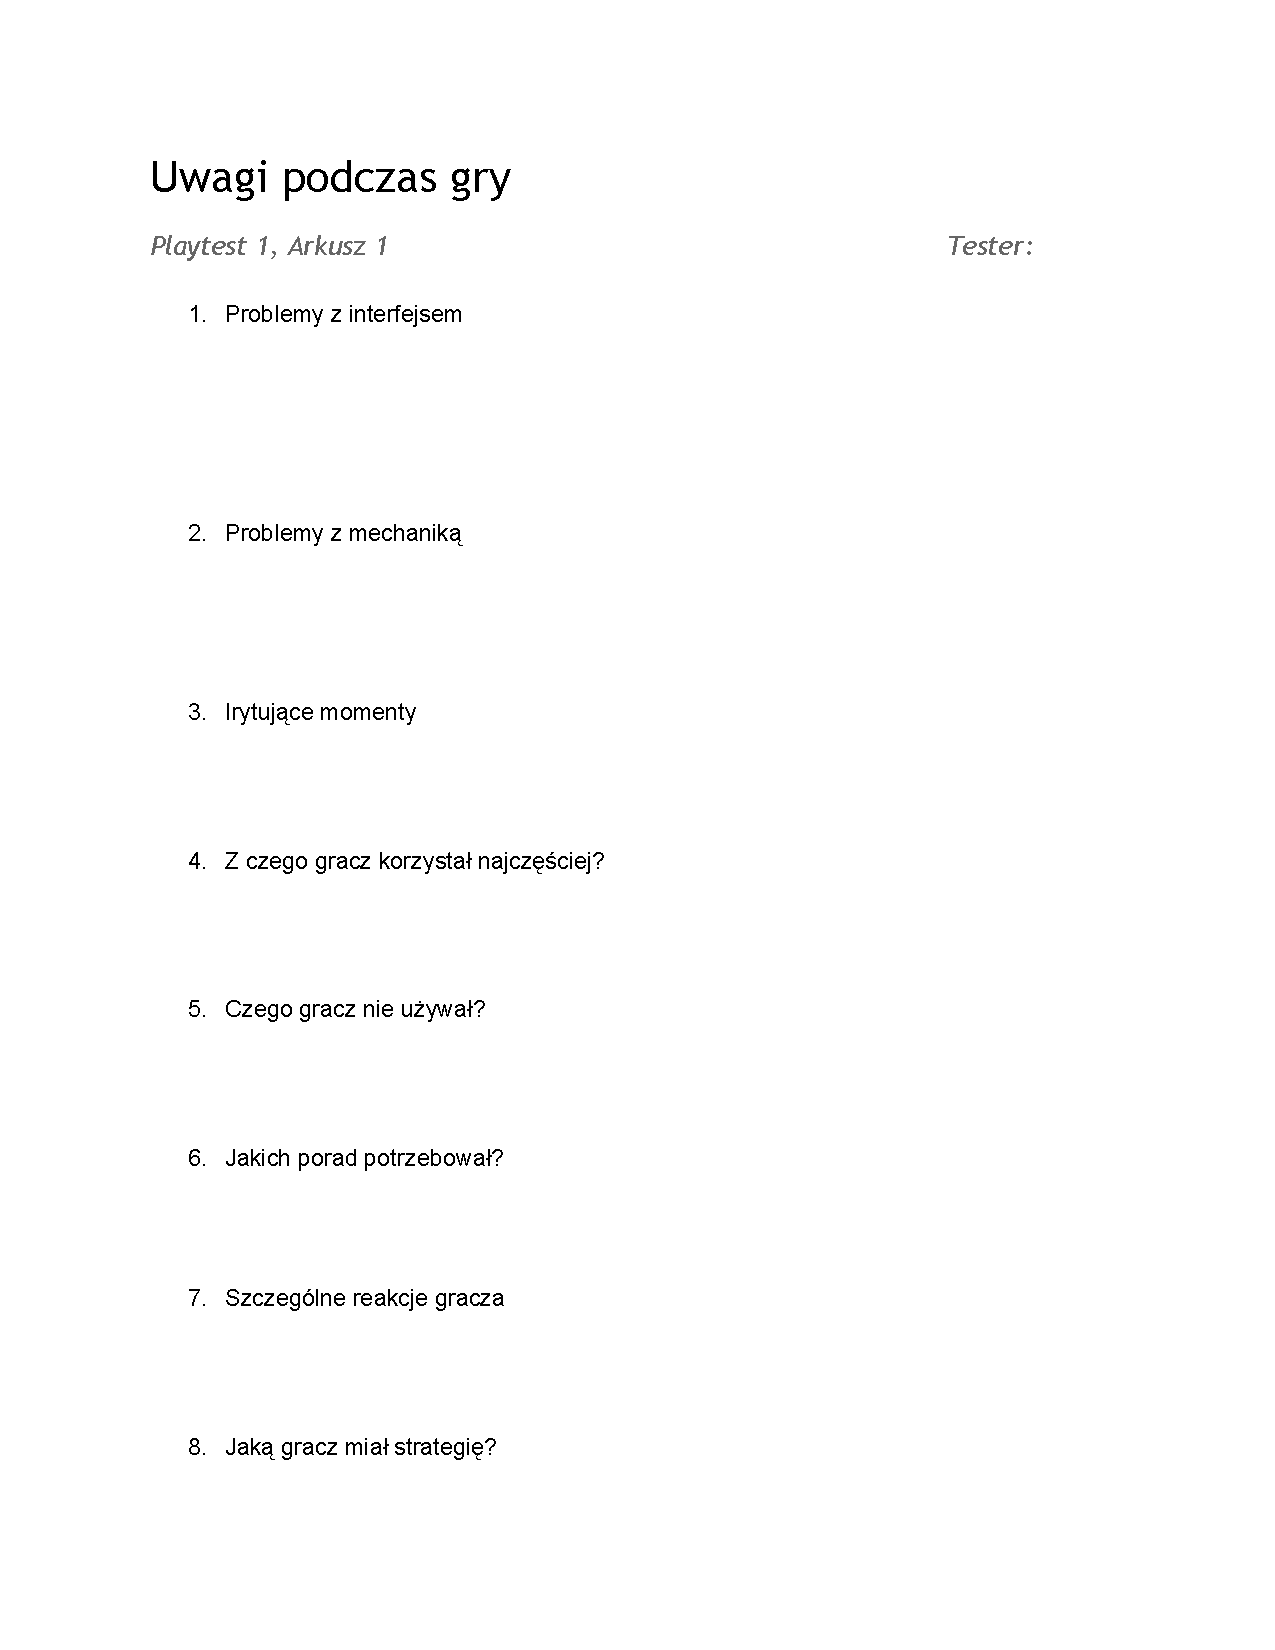
\includepdf[pages={-}]{Formularze-playtesty.pdf}
    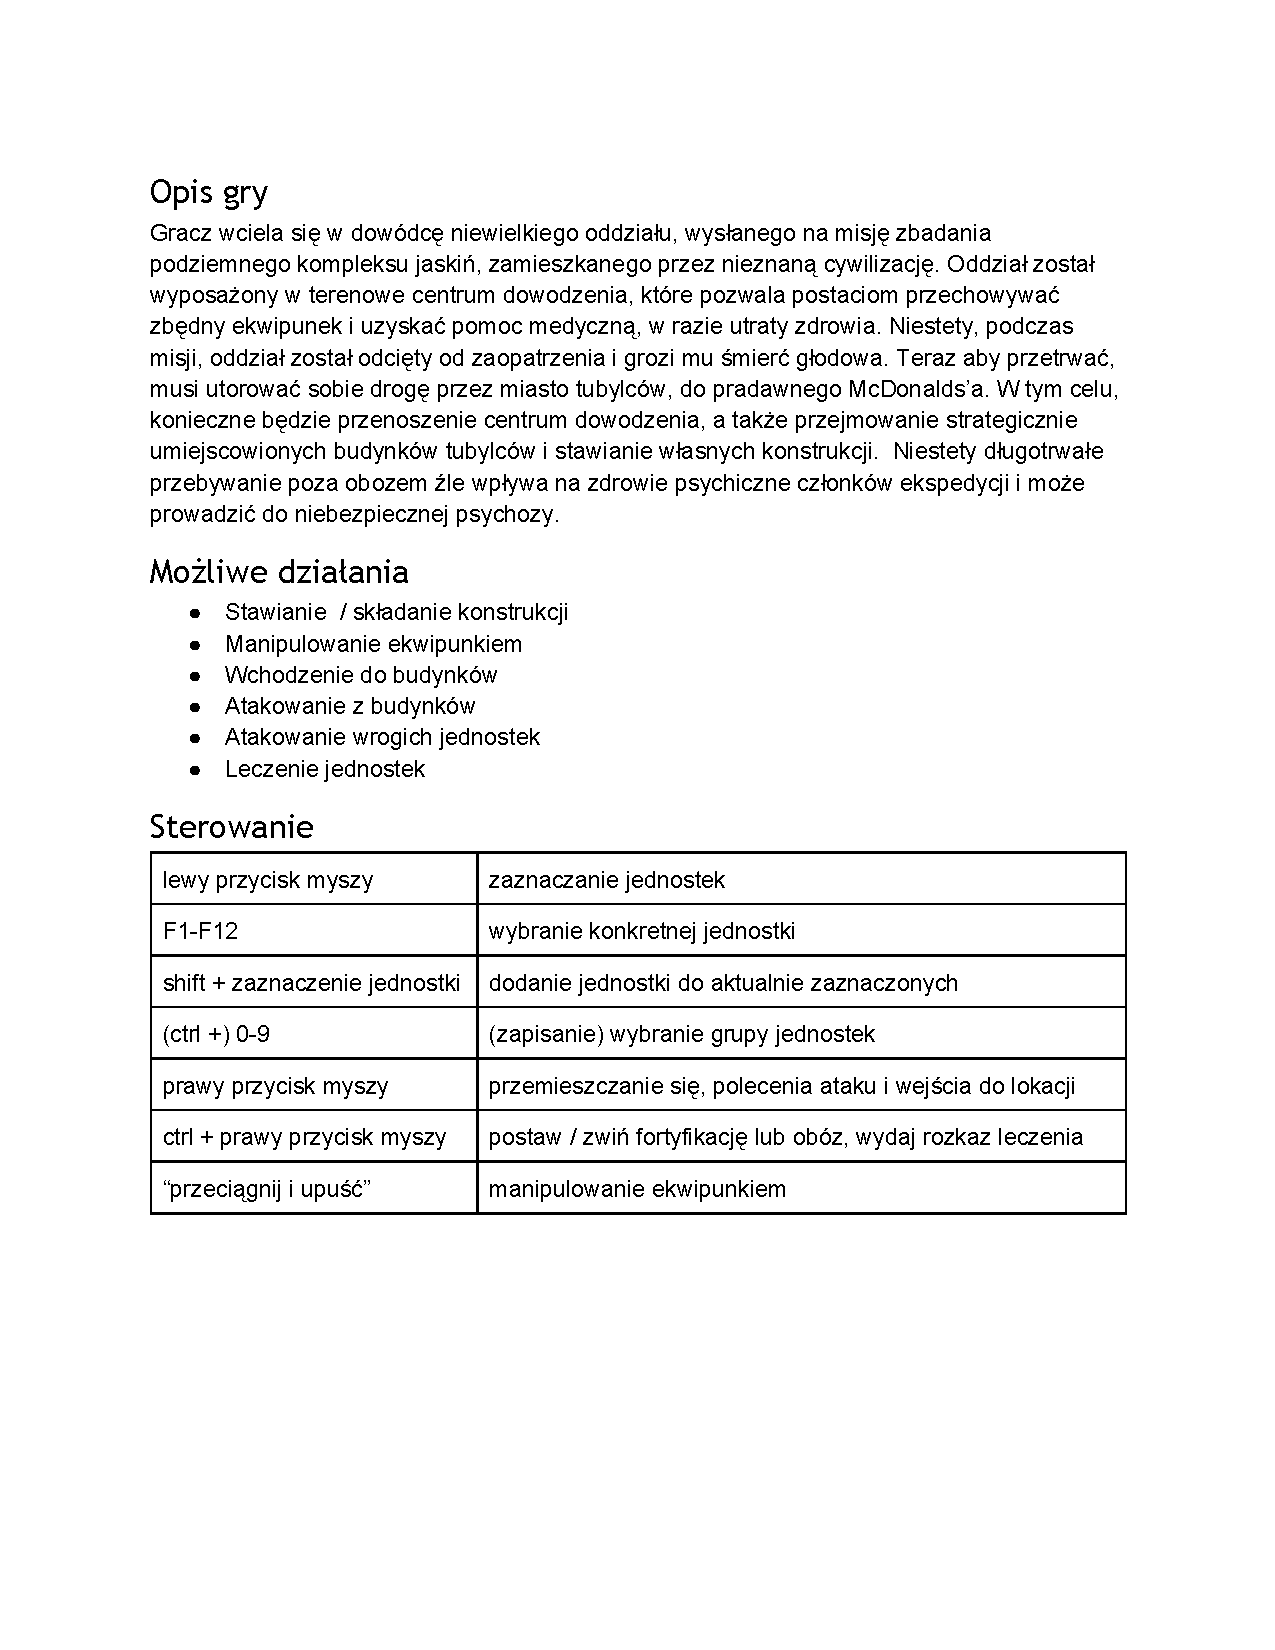
\includepdf[pages={-}]{Instrukcje-do-playtestow.pdf}
    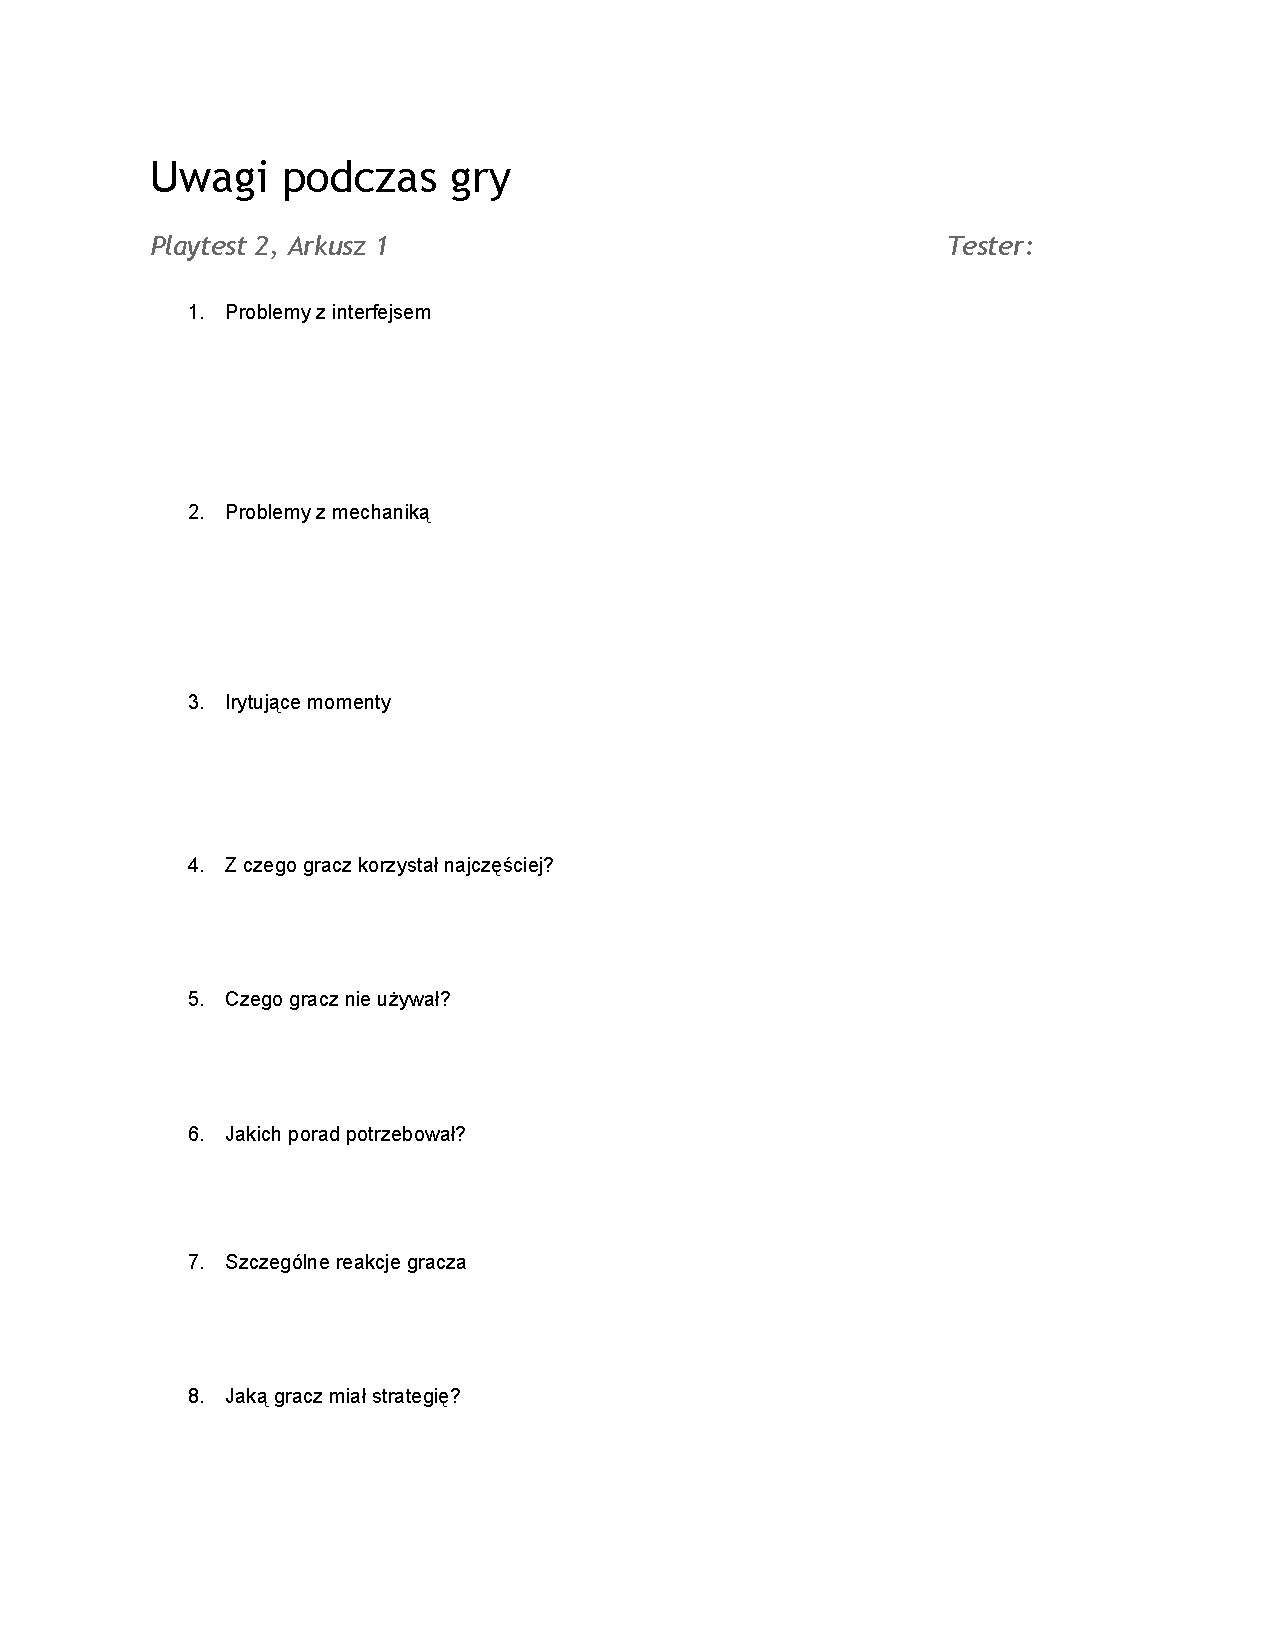
\includepdf[pages={-}]{Formularze-playtesty2.pdf}

  \chapter{Zawarość płyty CD}


\begin{thebibliography}{99}
\addcontentsline{toc}{chapter}{Bibliografia}
  %% To trzeba uładnić
  \item{\url{http://en.wikipedia.org/wiki/Gaussian_blur}}
  \item{\url{http://en.wikipedia.org/wiki/A*_search_algorithm}}
  \item{BOTEA, Adi; MÜLLER, Martin; SCHAEFFER, Jonathan. Near optimal hierarchical path-finding.
      Journal of game development, 2004, 1.1: 7-28.}
  \item{\url{http://doc.qt.io/qt-5/reference-overview.html}}

\end{thebibliography}

\end{document}


%%% Local Variables:
%%% mode: latex
%%% TeX-master: t
%%% coding: utf8
%%% End:
